% !Mode:: "TeX:UTF-8"

\def\xuewei{Doctor} % 默认
\documentclass[cs4size,openany,oneside,UTF8,nofonts]{ctexbook}
% \usepackage[a4paper,text={160true mm,234true mm},top=30.5true mm,left=25true mm,head=5true mm,headsep=2.5true mm,foot=8.5true mm]{geometry}
\usepackage[a4paper,text={170true mm,246.2true mm},top=25.4true mm,left=20true mm,head=5true mm,headsep=2.5true mm,foot=7.5true mm]{geometry}
\usepackage{ccaption}
\usepackage{booktabs}
\usepackage{longtable}
\usepackage{caption}
\usepackage{amsmath}
\usepackage{amssymb}
\usepackage{mathtools}
\usepackage{bigints}
\usepackage{bm}
\usepackage{txfonts}
\usepackage{graphicx}
\usepackage{enumitem}
\usepackage{fancyhdr}
\usepackage{ntheorem}
\usepackage{titlesec}
\usepackage{titletoc}                   % 控制目录的宏包
\usepackage{subfigure}
\usepackage{tabularx}
\usepackage[sort&compress,numbers]{natbib}
% \usepackage[boxed,linesnumbered,algochapter]{algorithm2e}	
\usepackage[ruled,linesnumbered]{algorithm2e}
% \usepackage{algorithmic}
\usepackage{listings}
\usepackage{lmodern}
\usepackage{tcolorbox}
\usepackage{tikz}
%
\usetikzlibrary{calc}
\lstset{ columns=flexible, breaklines=true }

\usepackage[xetex,
            bookmarksnumbered=true,
            bookmarksopen=true,
            colorlinks=false,
            pdfborder={0 0 1},
            citecolor=blue,
            linkcolor=red,
            anchorcolor=green,
            urlcolor=blue,
            breaklinks=true,
            naturalnames  %与algorithm2e宏包协调
            ]{hyperref}
\defaultfontfeatures{Mapping=tex-text}
\xeCJKsetemboldenfactor{1}%只对随后定义的CJK字体有效
\setCJKfamilyfont{hei}{SimHei}
\xeCJKsetemboldenfactor{4}
\setCJKfamilyfont{song}{SimSun}
\xeCJKsetemboldenfactor{1}
\setCJKfamilyfont{fs}{FangSong}
\setCJKfamilyfont{kai}{KaiTi}
\setCJKfamilyfont{li}{LiSu}
\setCJKfamilyfont{xw}{STXinwei}
\setCJKmainfont{SimSun}
\setCJKsansfont{SimHei}
\setmainfont{Times New Roman}
\setsansfont{Arial}
\newcommand{\heiti}{\CJKfamily{hei}}% 黑体   (Windows自带simhei.ttf)
\newcommand{\songti}{\CJKfamily{song}}    % 宋体   (Windows自带simsun.ttf)
\newcommand{\fs}{\CJKfamily{fs}}        % 仿宋体 (Windows自带simfs.ttf)
\newcommand{\kaishu}{\CJKfamily{kai}}      % 楷体   (Windows自带simkai.ttf)
\newcommand{\li}{\CJKfamily{li}}        % 隶书   (Windows自带simli.ttf)
\newcommand{\xw}{\CJKfamily{xw}}        % 隶书   (Windows自带simli.ttf)
\newfontfamily\arial{Arial}
\newfontfamily\timesnewroman{Times New Roman}
\setCJKfamilyfont{hwxk}{STXingkai}             %使用STXingkai华文行楷字体
\newcommand{\xingkai}{\CJKfamily{hwxk}}


\newcommand{\yihao}{\fontsize{26pt}{26pt}\selectfont}       % 一号, 1.倍行距
\newcommand{\xiaoyi}{\fontsize{24pt}{24pt}\selectfont}      % 小一, 1.倍行距
\newcommand{\erhao}{\fontsize{22pt}{1.25\baselineskip}\selectfont}       % 二号, 1.倍行距
\newcommand{\xiaoer}{\fontsize{18pt}{18pt}\selectfont}      % 小二, 单倍行距
\newcommand{\sanhao}{\fontsize{16pt}{16pt}\selectfont}      % 三号, 1.倍行距
\newcommand{\xiaosan}{\fontsize{15pt}{15pt}\selectfont}     % 小三, 1.倍行距
\newcommand{\sihao}{\fontsize{14pt}{14pt}\selectfont}       % 四号, 1.0倍行距
\newcommand{\xiaosi}{\fontsize{12pt}{12pt}\selectfont}      % 小四, 1.倍行距
\newcommand{\wuhao}{\fontsize{10.5pt}{10.5pt}\selectfont}   % 五号, 单倍行距
\newcommand{\xiaowu}{\fontsize{9pt}{9pt}\selectfont}        % 小五, 单倍行距

\newcommand\litem[1]{\item{\heiti#1\hspace{1.5em}}}

\newenvironment{listitem}{\begin{enumerate}[label={(\arabic*)},itemindent=2em]}{\end{enumerate}}

% \usepackage[boxed,linesnumbered,algochapter]{algorithm2e}  % 算法的宏包,注意宏包兼容性,先后顺序为float、hyperref、algorithm(2e),否则无法生成算法列表
\renewcommand{\algorithmcfname}{算法}

%\usepackage{tikz,mathpazo}

%\usetikzlibrary{shapes.geometric, arrows}

\newcommand{\citeayu}[1]{\citeauthor{#1}~(\citeyear{#1})\citeup{#1}}

\begin{document}

\titleformat{\chapter}{\center\xiaoer\hei}{\chaptertitlename}{0em}{}
\titlespacing{\chapter}{0pt}{0.5\bseieskip}{0.5\bseieskip}
\titleformat{\section}{\xiaosan\hei}{\thesection}{0em}{}
\titlespacing{\section}{0pt}{0.5\bseieskip}{0.5\bseieskip}
\titleformat{\subsection}{\sihao\hei}{\thesubsection}{0em}{}
\titlespacing{\subsection}{0pt}{0.5\bseieskip}{0.5\bseieskip}
\titleformat{\subsubsection}{\xiaosi\hei}{\thesubsubsection}{0em}{}
\titlespacing{\subsubsection}{0pt}{0pt}{0pt}

\newif\ifxueweidoctor
\newif\ifxueweimaster
\def\temp{Doctor}
\ifx\temp\xuewei
  \xueweidoctortrue  \xueweimasterfalse
\fi
\def\temp{Master}
\ifx\temp\xuewei
  \xueweidoctorfalse  \xueweimastertrue
\fi

% !Mode:: "TeX:UTF-8"
\setlength{\subfigbottomskip}{0pt}
\CTEXoptions[bibname={国内外主要参考文献}]
\CTEXsetup[name={,},number={}]{chapter}
\captionsetup{labelsep=space,font=small,justification=centering}
\arraycolsep=1.7pt
\graphicspath{{figures/}}
\renewcommand{\subcapsize}{\zihao{5}}
\renewcommand{\thesubfigure}{\alph{subfigure})}
\setcounter{secnumdepth}{4}
\newcommand{\pozhehao}{\raisebox{0.1em}{------}}
\titleformat{\chapter}{\center\zihao{-2}\heiti}{\chaptertitlename}{0.5em}{}
\titlespacing{\chapter}{0pt}{-4.5mm}{8mm}
\titleformat{\section}{\zihao{-3}\heiti}{\thesection}{0.5em}{}
\titlespacing{\section}{0pt}{4.5mm}{4.5mm}
\titleformat{\subsection}{\zihao{4}\heiti}{\thesubsection}{0.5em}{}
\titlespacing{\subsection}{0pt}{4mm}{4mm}
\titleformat{\subsubsection}{\zihao{-4}\heiti}{\thesubsubsection}{0.5em}{}
\titlespacing{\subsubsection}{0pt}{0pt}{0pt}
\makeatletter
\renewcommand\thesection{\@arabic \c@section} % 前面不带 thechapter
\makeatother

\theoremstyle{plain}
\theorembodyfont{\songti\rmfamily}
\theoremheaderfont{\heiti\rmfamily}
\newtheorem{definition}{\heiti 定义}
\newtheorem{example}{\heiti 例}
\newtheorem{algo}{\heiti 算法}
\newtheorem{theorem}{\heiti 定理}
\newtheorem{axiom}{\heiti 公理}
\newtheorem{proposition}{\heiti 命题}
\newtheorem{lemma}{\heiti 引理}
\newtheorem{corollary}{\heiti 推论}
\newtheorem{remark}{\heiti 注解}
\newenvironment{proof}{\noindent{\heiti 证明:}}{\hfill $ \square $ \vskip 4mm}
\theoremsymbol{$\square$}

% 定义页眉和页脚 使用fancyhdr 宏包
% \newcommand{\makeheadrule}{
% \rule[7pt]{\textwidth}{0.75pt} \\[-23pt]
% \rule{\textwidth}{0.75pt}}
% \renewcommand{\headrule}{
%     {\if@fancyplain\let\headrulewidth\plainheadrulewidth\fi
%      \makeheadrule}}
\fancypagestyle{plain}{%
\fancyhf{} % clear all header and footer fields
\fancyfoot[C]{\fontsize{9pt}{9pt}\selectfont\thepage} % except the center
\renewcommand{\headrulewidth}{0pt}
\renewcommand{\footrulewidth}{0pt}}
\pagestyle{plain}

\renewcommand{\CJKglue}{\hskip 0.56pt plus 0.08\baselineskip} %加大字间距,使每行33个字
\def\defaultfont{\renewcommand{\baselinestretch}{1.62}\normalsize\selectfont}
% 调整罗列环境的布局
\setitemize{leftmargin=3em,itemsep=0em,partopsep=0em,parsep=0em,topsep=-0em}
\setenumerate{leftmargin=3em,itemsep=0em,partopsep=0em,parsep=0em,topsep=0em}
\renewcommand{\theequation}{\arabic{equation}}
\renewcommand{\thetable}{\arabic{table}}
\renewcommand{\thefigure}{\arabic{figure}}

\makeatletter
\renewcommand{\p@subfigure}{\thefigure~}
\makeatother

\newcommand{\citeup}[1]{\textsuperscript{\cite{#1}}} % for WinEdt users

% 封面、摘要、版权、致谢格式定义
\makeatletter
\def\title#1{\def\@title{#1}}\def\@title{}
\def\titlesec#1{\def\@titlesec{#1}}\def\@titlesec{}
\def\affil#1{\def\@affil{#1}}\def\@affil{}
\def\subject#1{\def\@subject{#1}}\def\@subject{}
\def\researchdirection#1{\def\@researchdirection{#1}}\def\@researchdirection{}
\def\author#1{\def\@author{#1}}\def\@author{}
\def\bdate#1{\def\@bdate{#1}}\def\@bdate{}
\def\supervisor#1{\def\@supervisor{#1}}\def\@supervisor{}
\def\assosupervisor#1{\def\@assosupervisor{\textbf{副\hfill 导\hfill 师} & \rule[-4pt]{200pt}{1pt}\hspace{-326pt}\centerline{\textbf {#1}}\\}}\def\@assosupervisor{}
\def\cosupervisor#1{\def\@cosupervisor{\textbf{联\hfill 合\hfill 导\hfill 师} & \rule[-4pt]{200pt}{1pt}\hspace{-326pt}\centerline{\textbf {#1}}\\}}\def\@cosupervisor{}
\def\date#1{\def\@date{#1}}\def\@date{}
\def\stuno#1{\def\@stuno{#1}}\def\@stuno{}
% 定义封面
\ifxueweidoctor
\def\makecover{
    \thispagestyle{empty}
    \zihao{2}
		\renewcommand{\CJKglue}{\hskip 2pt plus 0.08\baselineskip}
    \centerline{\xingkai{中国科学技术大学}}
		\vspace{5mm}
		\centerline{\zihao{1}\songti\textbf{研究生学位论文开题报告}}
    \zihao{2}\vspace*{40mm}
		% \renewcommand{\CJKglue}{\hskip 2pt plus 0.08\baselineskip}
    % \centerline{\songti\textbf{题目:\rule[-4pt]{220pt}{1pt}\hspace{-220pt}\textbf\@title}}		
		% \centerline{\hspace{10em}\songti\textbf{\textbf\@titlesec}}		
    % \zihao{3}\vspace{4\baselineskip}
    \hspace*{-20pt}
    {\songti
	\renewcommand{\arraystretch}{1.1}
    \begin{tabular}{l@{}l}
    {论文题目}      & \rule[-4pt]{300pt}{1pt}\hspace{-390pt}\centerline{\@title}\\
    {}             & \rule[-4pt]{300pt}{1pt}\hspace{-390pt}\centerline{\@titlesec}\\
    {学生姓名}      & \rule[-4pt]{300pt}{1pt}\hspace{-390pt}\centerline{\@author}\\
    {学生学号}  & \rule[-4pt]{300pt}{1pt}\hspace{-390pt}\centerline{\@stuno}\\
    {指导老师}     & \rule[-4pt]{300pt}{1pt}\hspace{-390pt}\centerline{\@supervisor}\\
    {所在院系}   & \rule[-4pt]{300pt}{1pt}\hspace{-390pt}\centerline{\@affil}\\
    {学科专业}     & \rule[-4pt]{300pt}{1pt}\hspace{-390pt}\centerline{\@subject}\\
    {研究方向}     & \rule[-4pt]{300pt}{1pt}\hspace{-390pt}\centerline{\@researchdirection}\\
    {填表日期} & \rule[-4pt]{300pt}{1pt}\hspace{-390pt}\centerline{\@date}\\
    \end{tabular}\renewcommand{\arraystretch}{1}}
  \vfill
    \centerline{\zihao{-3}\kaishu{中国科学技术大学研究生院培养办公室}}
    \vspace{0.1\baselineskip}
    \centerline{\zihao{-3}\kaishu{二零零四年五月制表}}

%定义内封
    %新版本没有内封
\newpage
\thispagestyle{empty}
\begin{center}
 \heiti\zihao{2}{说\hspace{1em}明}
\end{center}
\vspace*{40pt}
   {\kaishu\zihao{3}

   \noindent 1.	抓好研究生学位论文开题报告工作是保证学位论文质量的一个重要环节。为加强对研究生培养的过程管理,规范研究生学位论文的开题报告,特印发此表。
   
   \vspace*{20pt}
   
   \noindent 2.	研究生一般应在课程学习结束之后的第一个学期内主动与导师协商,完成学位论文的开题报告。
   
   \vspace*{20pt}
   
   \noindent 3.	研究生需在学科点内报告,听取意见,进行论文开题论证。
   
   \vspace*{20pt}
   
   \noindent 4.	研究生论文开题论证通过后,在本表末签名后将此表交所在学院教学办公室备查。

   }
	\renewcommand{\arraystretch}{1}
    \clearpage
}
\fi

\ifxueweimaster
\def\makecover{
    \thispagestyle{empty}
    \zihao{-2}\vspace*{10mm}
		\renewcommand{\CJKglue}{\hskip 2pt plus 0.08\baselineskip}
    \centerline{\kaishu\textbf{中国科学技术大学}}
		
		\vspace{10mm}
		\centerline{\zihao{2}\songti\textbf{硕士学位论文开题报告}}

		\renewcommand{\CJKglue}{\hskip 0pt plus 0.08\baselineskip}
\vspace{30pt}
\zihao{-2}
\begin{center}\songti\textbf{题~目:\@title}\end{center}
\vspace{30pt}
    \zihao{3}
    \hspace*{68pt}{\songti
	\renewcommand{\arraystretch}{1.3}
    \begin{tabular}{l@{}l}
    \textbf{院\hfill (系)}   & \rule[-4pt]{200pt}{1pt}\hspace{-326pt}\centerline{\textbf\@affil}\\
    \textbf{学\hfill 科}     & \rule[-4pt]{200pt}{1pt}\hspace{-326pt}\centerline{\textbf\@subject}\\
    \textbf{导\hfill 师}     & \rule[-4pt]{200pt}{1pt}\hspace{-326pt}\centerline{\textbf\@supervisor}\\
    \@assosupervisor
	\@cosupervisor
    \textbf{研\hfill 究\hfill 生}      & \rule[-4pt]{200pt}{1pt}\hspace{-326pt}\centerline{\textbf\@author}\\
    \textbf{学\hfill 号}  & \rule[-4pt]{200pt}{1pt}\hspace{-326pt}\centerline{\textbf\@stuno}\\
    \textbf{开题报告日期} & \rule[-4pt]{200pt}{1pt}\hspace{-326pt}\centerline{\textbf\@date}\\
    \end{tabular}
		\renewcommand{\arraystretch}{1}}
	\vfill
    \centerline{\songti\textbf{研究生院培养处制}}

%%定义内封
\newpage
\thispagestyle{empty}
\zihao{5}\vspace*{2em}
\begin{center}
  \heiti\zihao{3}说\hspace{3em}明
\end{center}
\vspace*{40pt}
	\renewcommand{\arraystretch}{1.25}
    {\songti\zihao{5}
    \hangindent=2em
	\noindent 一、开题报告应包括下列主要内容:
    \begin{enumerate}[leftmargin=36pt]
	\item 课题来源及研究的目的和意义;
	\item 国内外在该方向的研究现状及分析;
	\item 主要研究内容;
	\item 研究方案及进度安排,预期达到的目标;
	\item 为完成课题已具备和所需的条件和经费;
	\item 预计研究过程中可能遇到的困难和问题,以及解决的措施;
	\item 主要参考文献。
    \end{enumerate}
    \noindent 二、对开题报告的要求
	\begin{enumerate}[leftmargin=36pt]
	\item 开题报告的字数应在~5000~字以上;
	\item 阅读的主要参考文献应在~20~篇以上,其中外文资料应不少于三分之一。硕士研究生应在导师的指导下着重查阅近年内发表的中、\hspace{-1pt}外文期刊文章。\hspace{-1pt}本学科的基础和专业课教材一般不应列为参考资料。
    \end{enumerate}
    \noindent 三、开题报告时间应最迟不得超过第三学期的第三周末。

    \hangindent=2em\noindent 四、如硕士生首次开题报告未通过,\hspace{-2pt}需在一个月内再进行一次。\hspace{-3pt}若仍不通过,\hspace{-2pt}则停止硕士论文工作。

    \noindent 五、此表不够填写时,可另加附页。

\hangindent=2em\noindent 六、开题报告进行后,此表同硕士学位论文开题报告评议结果存各系(院)研究生秘书书处,以备研究生院及所属学院进行检查。

    }
	\renewcommand{\arraystretch}{1}
    \clearpage
}
\fi
\makeatother

% !Mode:: "TeX:UTF-8"

\affil{计算机科学与技术}
\subject{计算机应用技术}
\researchdirection{xxxxx}
\author{陈xx}
\supervisor{陈xx \enspace 教授}
% \assosupervisor{副导名}%若无副导师,请屏蔽掉此句
% \cosupervisor{联导名}%若无联合导师,请屏蔽掉此句
\date{2019年12月25日}
\stuno{BA1xxxxxxxx}
\bdate{2004年5月}

\ifxueweidoctor
  \title{基于xxxxxxxxxxx} %论文题目
  \titlesec{xxxxx研究与实现}

\makecover
\clearpage
\setcounter{page}{1} 
\zihao{-4}
% \tableofcontents    % 中文目录
% \chapter*{基于xxxxxxxxxxxxxxxxxx研究与实现}

%\animategraphics[height=2.8in,autoplay,loop,controls]{12}{animate_}{0}{22}
% \input{body/figures}
% \input{body/tables}
% \input{body/equations}
% \input{body/others}
\section{选题依据}

%%%%%%%%%%%% 画框, 每页自己调节
\begin{tikzpicture}[overlay,remember picture]
  \draw [line width=0.8pt]
      ($ (current page.north west) + (1.8cm,-3.5cm) $)
      rectangle
      ($ (current page.south east) + (-1.8cm,2.5cm) $);
\end{tikzpicture}
%%%%%%%%%%%% 画框, 每页自己调节

图片例子,如图 \ref{图片例子}
\begin{figure}[htbp]
  \centering
  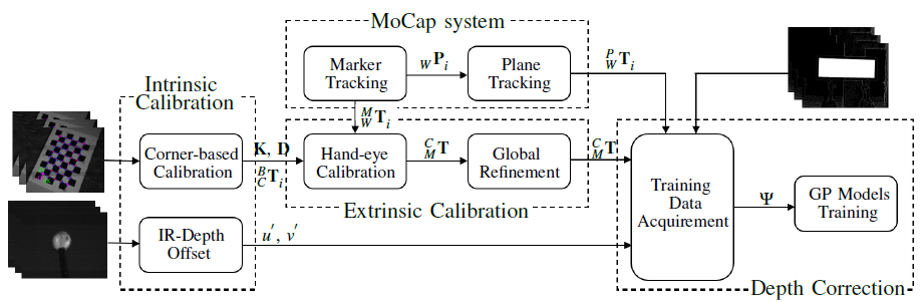
\includegraphics[width = 0.7\textwidth]{rgbd_1.png}
  \caption{图片例子}\label{图片例子}
  \vspace{-1em}
\end{figure}

算法例子:算法\ref{alg1}
\begin{algorithm}
  \caption{算法例子}
  \label{alg1}
  Initialize policy network $\pi_\theta$ and value function $V_\phi (s_t)$.

  \For{epoch $ = 1,2...,$}
  {
          \textit{// ...}

          $\pi_{old} \leftarrow \pi_{\theta}$

          \textit{// Update policy network}
          
          \For{$m = 1,...,E_{\pi}$}
          {
                  $L^{PPO}(\theta) = \sum_{t=1}^{T_{max}}{min(\frac{\pi_{\theta}(a_{i}^{t}|o_{i}^{t})}
                  {\pi_{old}(a_{i}^{t}|o_{i}^{t})}\hat{A}_{i}^{t}, 
                  clip(\frac{\pi_{\theta}(a_{i}^{t}|o_{i}^{t})}{\pi_{old}(a_{i}^{t}|o_{i}^{t})},1-\varepsilon ,1+\varepsilon )
                  \hat{A}_{i}^{t})}$

                  \If {KL$[\pi_{old} | \pi_{\theta}] > 1.5{KL}_{target}$}
                  {
                          \textbf{break}
                  }
                  Update $\theta$ with $lr_{\theta}$ by Adam w.r.t $L^{PPO}(\theta)$.
          }

          \textit{// Update value function}

          \For{$n = 1,...,E_{V}$}
          {
                  $L^{V}(\phi) = -\sum_{N}^{i=1}\sum_{t=1}^{T_i}(\sum_{t'>t}\gamma ^{t'-t}r_{i}^{t'} - V_{\phi}(s_i^t))^2$

                  Update $\phi$ with $lr_{\phi}$ by Adam w.r.t $L^{V}(\phi)$.
          }

  }
\end{algorithm}

公式例子
\begin{equation}
  \textbf{M}_t = f_{\lambda}(s_t)
\end{equation}
\begin{equation}
  a_{t} = \pi_{\theta}(\textbf{M}_t, g_t, v_t, {\omega}_t)
\end{equation}

\newpage
%%%%%%%%%%%% 参考文献引用
哈哈哈哈哈哈哈 \cite{陈赢峰机器人导航的研究}
%%%%%%%%%%%% 画框, 每页自己调节
\begin{tikzpicture}[overlay,remember picture]
  \draw [line width=0.8pt]
      ($ (current page.north west) + (1.8cm,-2.3cm) $)
      rectangle
      ($ (current page.south east) + (-1.8cm,2.5cm) $);
\end{tikzpicture}
%%%%%%%%%%%% 画框, 每页自己调节
\newpage
%%%%%%%%%%%% bib参考文献
\bibliographystyle{GBT7714-2005NLang-HIT}
\addtolength{\bibsep}{-0.8em}
\nocite{*}
\bibliography{reference}

\newpage
\section{已取得的与论文研究内容相关的成果}
\subsection{论文成果}
\begin{itemize}
  \item \textbf{Guangda Chen}, Guowei Cui, Zhongxiao Jin, Feng Wu, and Xiaoping Chen. (2019). Accurate Intrinsic and Extrinsic Calibration 
  of RGB-D Cameras with GP-based Depth Correction. \textit{IEEE SENSORS JOURNAL}. (SCI三区,IF: 3.076)
\end{itemize}
\subsection{比赛成果}
\begin{table}[!htbp]
  \vspace{-0.5em}\label{table1}\centering\zihao{5}
  \begin{tabular}{llll}
  \toprule
  时间 & 名称 & 地点 & 奖项\\
  \midrule
  2019.08 & IJCAI-2019 养老机器人挑战赛 & 中国澳门 & 第一名\\
  2017.07 & RoboCup2017@Home & 日本名古屋 & 最佳操作奖\\
  2016.07 & RoboCup2016@Home & 德国莱比锡 & 第三名\\
  2015.09 & 2015年全国机器人大赛 & 中国贵阳 & 第一名\\
  \bottomrule
  \end{tabular}
\end{table}
\begin{tikzpicture}[overlay,remember picture]
  \draw [line width=0.8pt]
      ($ (current page.north west) + (1.8cm,-3.5cm) $)
      rectangle
      ($ (current page.south east) + (-1.8cm,2.5cm) $);
\end{tikzpicture}

%%%% 以下小节根据内容更改,没有和官方目录一致
\newpage
\section{研究内容与目标}

\section{技术路线与可行性分析}

\section{已有的科研进展}

\section{创新点总结}

\section{研究计划与安排}

%%%% 签名
\vspace*{10pt}
\rightline{研究生本人签名:\underline{\hbox to 61mm{}}}
\vspace*{10pt}
\rightline{\qquad \qquad 年\qquad \qquad 月\qquad \qquad 日}
\end{document}
